\documentclass[a5paper,12pt]{memoir}
\semiisopage
\medievalpage[12]
%\chapterstyle{madsen}
\setlength{\headwidth}{0.8\textwidth}
\addtolength{\headwidth}{\marginparsep}
\addtolength{\headwidth}{\marginparwidth}
\pagestyle{companion}
\usepackage{graphicx,caption}
\usepackage{amssymb,amsmath,amsthm}
\usepackage[T2A]{fontenc}
\usepackage[utf8]{inputenc}
\usepackage[russian]{babel}
\usepackage{indentfirst}
\usepackage{enumitem}
\usepackage{wrapfig}
%\usepackage{statmodtitle}
\usepackage[top=1.5cm,bottom=1.5cm]{geometry}
\graphicspath{{images/}}
\newtheorem{definition}{Определение}
\newtheorem{axiom}{Постулат}
\newtheorem{theorem}{Теорема}
\newtheorem{example}{Пример}
\newtheorem{task}{Задача}
\newcommand{\solution}{\proof[Решение]}

\title{Физика в ЛШ СУНЦ НГУ}
%\author{Рабусов Андрей}
\date{\today}
%\subtitle{Курсовая работа, атомный практикум}
%\chief{Эйдельман Семён Исаакович}
%\setlength{\topmargin}{-5mm}
%\setlength{\textwidth}{15.7cm}
\includeonly{abstract,math-intro,kinematics,dynamics,statics,save-laws}
\begin{document}
\maketitle
\begin{abstract}
Пособие содержит краткий теоретический материал по школьной механике,
а также задачи и примеры, необходимые для освоения базовых
понятий физики. Кроме этого, пособие содержит математическое
введение, необходимость в котором возникает из-за несинхронизованности
программ по математике и физике.
Предназначается для семинарских занятий по физике
в девятых классах
летней школы СУНЦ НГУ.\end{abstract} 

\newpage
\tableofcontents
\chapter{Математический минимум}
\subsection*{Обозначения}
\begin{description}
\item[$\in$] --- принадлежит
\item[$\subset$] --- является подмножеством,
\item[$\forall$] --- для любого,
\item[$\exists$] --- существует,
\item[$\Rightarrow$] --- следует,
\item[$|\cdot|$] --- абсолютное значение (модуль),
\item[$\amalg$] --- пусть (квантор попустительства).
\end{description}
\section{Функции}
\begin{definition}[Функция]
Пусть есть числовые множества $X=\mathbb{D}(f) \subset \mathbb{R}$ 
(область определения) и $Y=\mathbb{E}(f) \subset \mathbb{R}$ (множество
значений). Каждому $x\in X$ сопоставим \textbf{единственный} $y\in Y$.
\end{definition}
\begin{definition}[Полный образ функции]
$$\mathbf{Im} f = \{ f (x)~|~\forall x \in X \}$$
\end{definition}
\begin{definition}[Наложение (сюръекция)]
$$Y=\mathbf{Im} f$$
\end{definition}
В дальнейшем под словом <<функция>> будем подразумевать наложение. Если область определения
функции явно не указана, то будем подразумевать под $X$ естественную область определений ---
множество таких $x \in \mathbb {R}$, что выражение $f(x)$ определено.
\begin{definition}[Чётная функция]
$$\forall x \in X \Rightarrow -x \in X $$
$$f(x) = f(-x)$$
\end{definition}
\begin{example}[Пример чётных функций]
$$x^{2k},~k\in \mathbb{Z};~\cos x;~\ch x $$
\end{example}
\begin{definition}[Нечётная функция]
$$\forall x \in X \Rightarrow -x \in X $$
$$f(-x) = -f(x)$$
\end{definition}
\begin{example}[Пример нечётных функций]
$$x^{2k-1},~k\in\mathbb{Z};~\sin x;~\sh x $$
\end{example}
\begin{definition}[Монотонно возрастающая функция]
$$x_1~,x_2 \in X,~x_1 < x_2 \Rightarrow f(x_1) < f(x_2)$$
\end{definition}
Аналогичным образом определяются монотонно  убывающая функция, невозрастающая и неубывающая функции.
\begin{definition}[Абсолютный максимум]
$$x_0 \in X,~\forall x \ne x_0 f(x) < f(x_0)$$
\end{definition}
\begin{definition}[Локальный максимум]
$$x_0 \in X,~x\in \mathbb{B} (x_0,\varepsilon),~\varepsilon > 0,~ f(x) < f(x_0),$$
где $\mathbb{B}(x_0,\varepsilon) = \{x \in X~|~x \ne x_0,~|x-x_0|<\varepsilon\}$
\end{definition}
Аналогично определяются абсолютный и локальный минимумы.
\begin{definition}[Обратная функция]
Если каждому значению $y \in Y$ функции $f$ соответствует не более одного (в случае наложения --- строго
один) $x \in X$, то можно постороить обратную функцию по следующему правилу:
$$\mathbb{D}f^{-1} = \mathbf{Im}(f)$$
$$\mathbb{E}f^{-1} = \mathbb{D}f$$
$$\forall y \in \mathbb{E}f,~f^{-1}(y)=x,~x \in X,$$
при этом
$$y=f(x)$$
\end{definition}
\begin{definition}[Периодическая функция]
Если $$\exists \xi > 0~|~\forall x \in X,~f(x+\xi)=f(x),$$
то функцию $f$ называют периодической, а $\xi$ --- периодом.
\end{definition}
\subsection*{Задачи}
\begin{task}
Найдите естественную область определений следуюущих функций:
$\frac{1}{a^2-x^2};$
$\frac{1}{a^2-(x-b)^2};$
$\frac{1}{a^2+(x-b)^2};$
$\frac{1}{a-\sqrt{x-b}},$ $a,~b \in \mathbb{R}.$
\end{task}
\begin{solution}
$x\in \mathbb{R},~x \ne \pm a; $
$x \in \mathbb{R},~x \ne \pm a+b; $
$x \in \mathbb{R};$
$x \in \mathbb{R},~x \ge b,$ в случае
$a \ge 0 \Rightarrow x \ne a^2 + b.$
\end{solution}
\begin{task}
Найдите полный образ следующих функций:
$f(x)=\frac{1}{a^2 + (x-b)^2},$
$f(x)=\frac{1}{a + \sqrt{x-b}},$
$f(x)=\frac{\sqrt{x-a}}{\sqrt{x-b}}.$
\end{task}
\begin{solution}
Задача с нахождением области значений 
\textit{непрерывной} функции
обычно сводится к нахождению
абсолютного минимума и максимума функции.
\begin{enumerate}
\item $f(x)$ можно представить как композицию функций $\frac {1}{x}$ и
$a^2 + (x-b)^2.$
Минимальное значение выражение
${a^2 + (x-b)^2}$ принимает при $x=b,$ максимальное значение
не существует, функция неограничена сверху. Значит $f(x)$ ограничена
снизу нулём.
Поэтому окончательно получаем
$Y=\{x\in\mathbb{R}~|~0<x\le \frac{1}{a^2}\}.$
\item Аналогично предыдущему пункту задачи рассмотрим сначала множество значений
знаменателя. Ясно, что это полуось $[a,~+\infty).$ В зависимости от того, содержит
ли ноль это множество, возникает два случая. Если $a>0$, то знаменатель в ноль
не обращается, функция непрерывна, её множество значений $(0,~\frac{1}{a}].$
Если $a=0$, то имеем $Y=(0,~+\infty).$
В случае $a<0$ разобьём множество значений на две части: знаменатель больше нуля
(это соответствует множеству $(0,~+\infty)$) и знаменатель меньше нуля
(соответствует $(-\infty,~\frac{1}{a}],$ где окончательно получим
$Y=(-\infty,~\frac{1}{a}]\cup(0,~+\infty).$
\item Случай $a=b$ тривиален, $Y=\{1\}.$ Случай $a>b$ рассмотрим подробнее.
Рассмотрим подкоренное выражение
($x\in X$). $$\frac{x-a}{x-b} = 1 - \frac {a-b}{x-b}<1.$$
Подкоренное выражение монотонно возрастает, значит монотонно возрастает и корень
из него (на области определений). Поэтому имеем $Y=[0,1).$ Если $a<b,$ то
подкоренная функция (а следовательно и сама функция) монотонно убывает на $X.$
В этом случае имеем $Y=(1,+\infty).$
\end{enumerate}
\end{solution}
\begin{task}
Найдите функцию, обратную $f(x)=ax^2+bx+c.$
\end{task}
\begin{solution}
Если за $X$ выбрать $[-\frac{b}{2a},~+\infty),$
то $f^{-1}(x) = \frac{-b+\sqrt{b^2-4a(c-x)}}{2a}$.
Если за $X$ выбрать $(-\infty,~-\frac{b}{2a}],$
то $f^{-1}(x) = \frac{-b-\sqrt{b^2-4a(c-x)}}{2a}$.
\end{solution}
\section{Тригонометрические функции}
Рассмотрим окружность единичного радиуса.
\begin{wrapfigure}{r}{0.5\textwidth}
 \begin{center}
  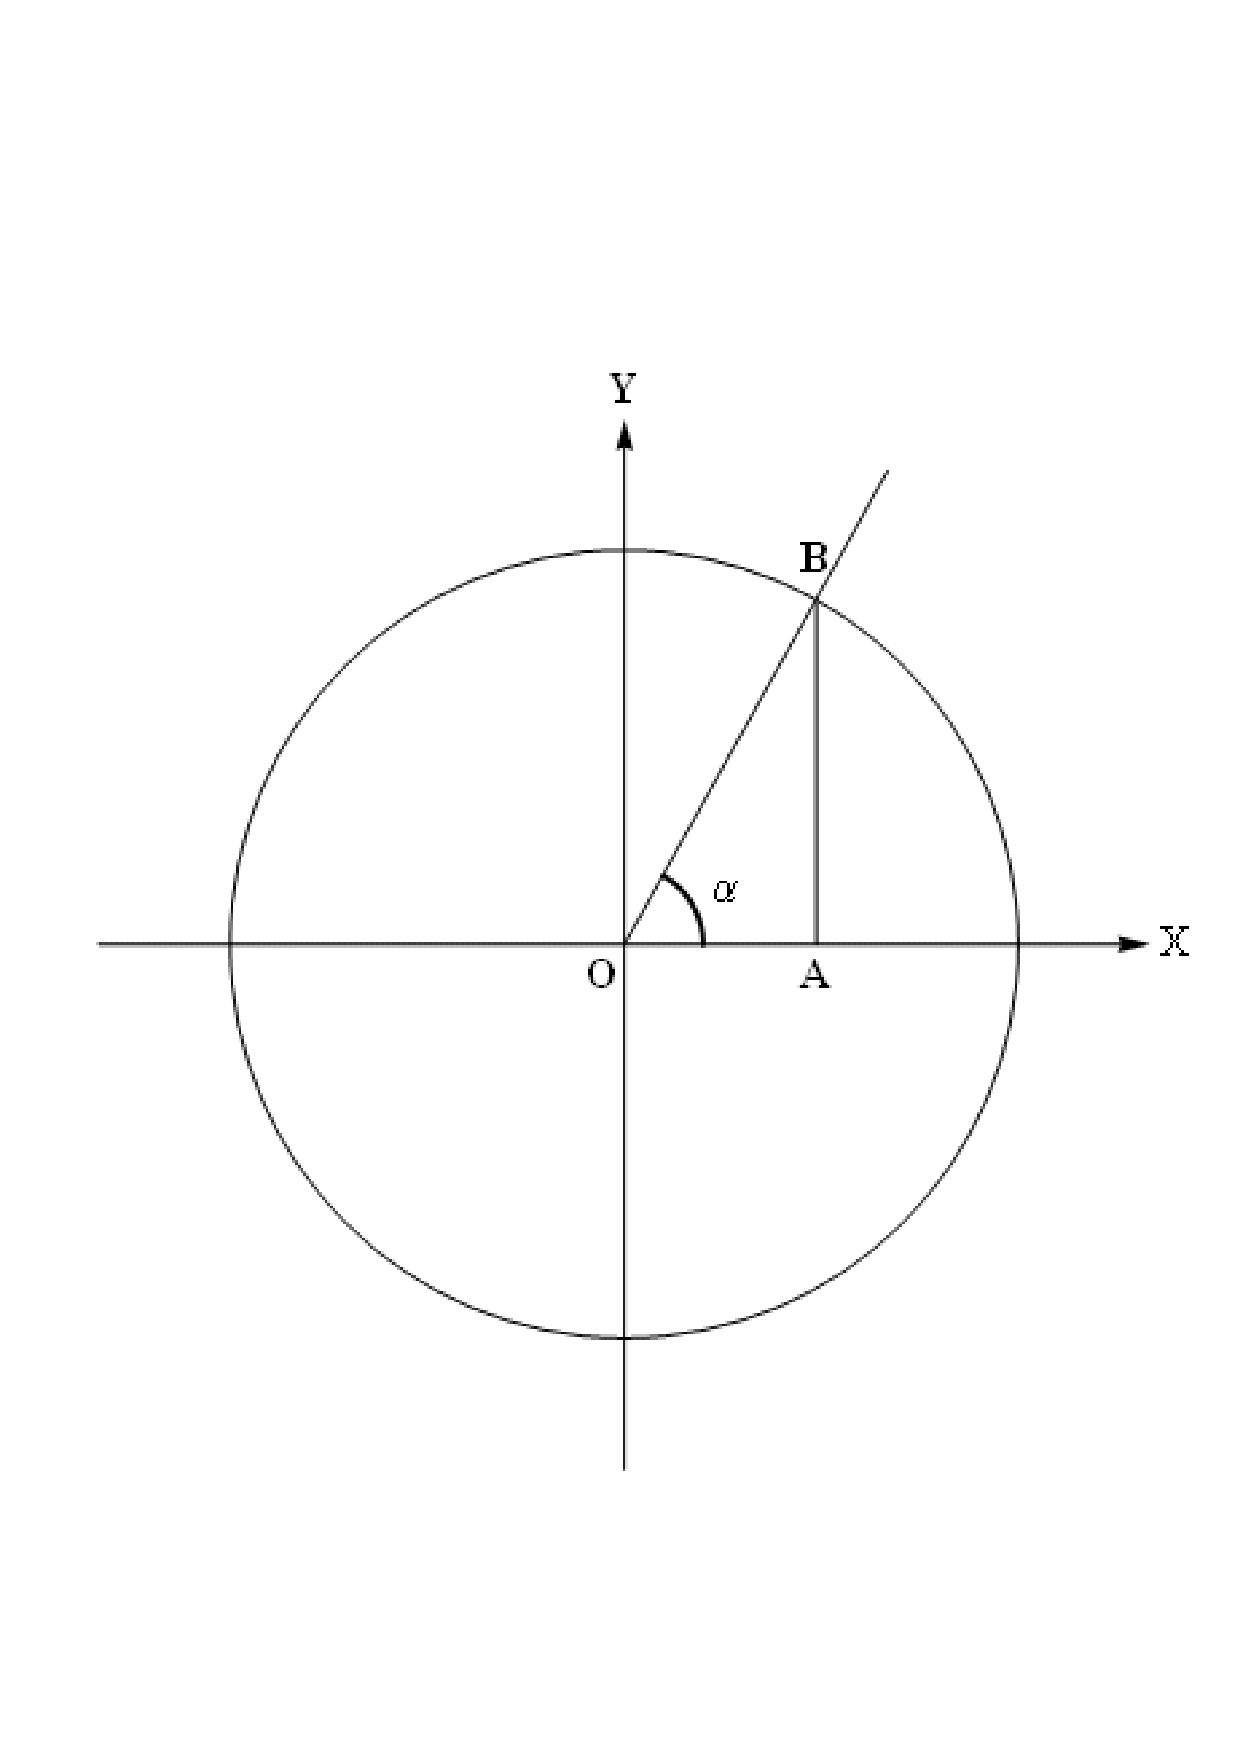
\includegraphics[width=0.48\textwidth]{trigonometry}
 \end{center}
 \caption{Единичная окружность}
 \label{pic:trig_circle}
\end{wrapfigure}
Введём систему декартовых
координат с нулём в центре окружности (точка $O$, рис.~\ref{pic:trig_circle}).
Отобразим числовую прямую на окружность,
а именно сопоставим ноль числовой прямой с точкой пересечения окружности и оси абсцисс (точка $A$).
Затем сопоставим точку $x$ числовой прямой с точкой на окружности, отложенной от
нулевой точки так, что длина полученной дуги окружности будет в точности равна $x$ (точка $B$).
Длина всей окружности равна $2\pi$ по определению числа $\pi,$ тогда очевидно,
что точки вида $x+2\pi k,~k\in \mathbb{Z}$ числовой прямой будут отображены в одну и ту же
точку на окружности. Значение угла $\angle BOA$ определим как длину дуги $\cup BOA.$ Теперь
определим тригонометрические функции.
\begin{definition}[Косинус]
$\cos x$ --- это $x$-координата точки $B.$
\end{definition}
\begin{definition}[Синус]
$\sin x$ --- это $y$-координата точки $B.$
\end{definition}
\begin{definition}[Тангенс]
$\tg x = \frac {\sin x}{\cos x}.$
\end{definition}
\begin{definition}[Котангенс]
$\ctg x = \frac {\cos x}{\sin x}.$
\end{definition}
Существуют такие функции, как $\sec x$ и $\csc x,$ но только бородатые старики,
запертые в подвалах университетов, помнят определение этих экзотических символов.
Самые базовые свойства тригонометрических функций мы рассмотрим в задачах, более
последовательно тригонометрия будет изложена в основном курсе математики ФМШ.
\subsection*{Задачи}
\begin{task}
Найдите период функций $\sin x,$ $\cos x,$ $\tg x,$ $\ctg x.$
\end{task}
\begin{solution}
$2\pi,~2\pi,~\pi,~\pi.$
\end{solution}
\begin{task}
Найдите область определения функций $\sin x,$ $\tg x.$
\end{task}
\begin{solution}
Проекция на ось $y$ определена всегда, поэтому
$\mathbb{D}\sin = \mathbb{R}.$
Функция $\cos x$ принимает значение $0$ при $x=\pi (k + 1/2), k \in \mathbb{Z}.$
Поэтому $\mathbb{D}\tg = \mathbb{R}\setminus\{\pi (k +1/2)\vert k\in\mathbb{Z}\}.$
\end{solution}
\begin{task}
Найдите область значений функций $\cos x,$ $\ctg x.$
\end{task}
\begin{solution}
Максимальное значение функции $\cos x$ --- $1$,
минимальное --- $-1,$ функция
\textit{непрерывна},
поэтому $\mathbb{E}\cos = [-1,~1].$
$\mathbb{E}\ctg = \mathbb{R}.$
\end{solution}
\begin{task}
Найдите значение функций $\sin x,$ $\tg x$
при $x =  0,$ 
$\pi/6,$ $\pi/4,$ $\pi/3,$ $\pi/2.$
\end{task}
\begin{solution}
$\sin x = 0,$ $1/2,$ $\sqrt 2/2,$ $\sqrt 3/2, 1.$
$\tg x = 0,$ $1/\sqrt 3,$ $1,$ $\sqrt 3,$ не определён.
\end{solution}
\begin{task}
Докажите следующие соотношения:
\begin{enumerate}
\item $\sin -x = -\sin x,$
\item $\sin (\pi/2-x) = \cos x,$
\item $\sin (x+\pi) = -\sin x,$
\item $\sin^2 x + \cos^2 x = 1.$
\end{enumerate}
\end{task}
\section{Понятие вектора}
Рассмотрим множество $\mathbb{V}$ элементов $\mathbf{v}.$ Пусть для всех $\mathbf{v}$ определена
бинарная операции (сложение) и операция умножения на скаляр (в нашем случае скаляром
будем считать элементом множества $\mathbb{R}$). Заданные операции удовлетворяют следующим
аксиомам 
($\mathbf{x},$ $\mathbf{y},$ $\mathbf{z} \in \mathbb{V},$ $\lambda, \mu \in \mathbb{R}$):
\begin{enumerate}
\item $\mathbf{x}+\mathbf{y} = \mathbf{y}+\mathbf{x},$
\item $\mathbf{x}+(\mathbf{y}+\mathbf{z}) = (\mathbf{x} + \mathbf{y}) + \mathbf{z},$
\item $\forall\mathbf{x}~\exists \mathbf{0} \in \mathbb{V}$ такой что $\mathbf{x}+\mathbf{0} = \mathbf{x},$
\item $\forall\mathbf{x}~\exists \mathbf{-x}\in\mathbb{V}$ такой что $\mathbf{x}+(\mathbf{-x})=\mathbf{0},$
\item $\lambda (\mu\mathbf{x}) = (\lambda \mu) \mathbf{x},$
\item $1\mathbf{x} = \mathbf{x},$
\item $(\lambda+\mu)\mathbf{x} = \lambda\mathbf{x} + \mu\mathbf{x},$
\item $\lambda (\mathbf{x} + \mathbf{y}) = \lambda \mathbf{x} + \lambda \mathbf{y}.$
\end{enumerate}
\begin{definition}[Векторное пространство]$\mathbb{V}.$\end{definition}
\begin{definition}[Вектор]$\mathbf{v} \in \mathbb{V}.$
 \label{def:vec}
\end{definition}
\begin{definition}[Линейная комбинация]
$\mathbf{L} = \sum\limits_{i=1}^{n}\lambda_i \mathbf{x}_i,$ $i \in \mathbb{N},$
$\lambda_i \in \mathbb{R},$ $\mathbf{x}_i\in\mathbb{V}.$
\end{definition}
\begin{definition}[Линейная независимость]
Система векторов $\{\mathbf{x}_i~\vert~\mathbf{x}_i\in \mathbb{V}\}$ является
линейнонезависимой, если $\mathbf{L}=0 \Leftrightarrow \forall i \therefore 1\le i\le n,$ $i\in\mathbb{N},$ 
$\lambda_i = 0.$
\end{definition}
\begin{definition}[Базис]
Система линейнонезависимых векторов $\{\mathbf{x}_i\}$ называется
базисом, если $\forall \mathbf{x} \in \mathbb{V}$ можно
представить в виде линейной комбинации $\{\mathbf{x}_i\}.$
\end{definition}
\begin{definition}[Размерность пространства]
$\dim \mathbb{V}$ --- число векторов в базисе.
\end{definition}
В физических задачах очень часто встречаются случаи, когда $\dim \mathbb{V} = 3.$
\begin{definition}[Скалярное произведение]
Бинарная операция $\langle \cdot \vert \cdot \rangle$ определена для всех
пар $\mathbf{x},$ $\mathbf{y} \in \mathbb{V},$ принимает значения из $\mathbb{R}$ и
удовлетворяет следующим условиям
при $\mathbf{x},$ $\mathbf{y},$ $\mathbf{z} \in \mathbb{V},$ $\lambda, \mu \in \mathbb{R}$:
\begin{enumerate}
\item $\langle \mathbf{x} \vert \lambda \mathbf{y} + \mu \mathbf{z} \rangle
 = \lambda \langle \mathbf{x} \vert \mathbf{y} \rangle
 + \mu \langle \mathbf{x} \vert \mathbf {z} \rangle,$
\item $\langle \mathbf{x} \vert \mathbf {y} \rangle
 = \langle \mathbf{y} \vert \mathbf {x} \rangle,$
\item $\langle \mathbf {x} \vert \mathbf {x} \rangle \ge 0,$
 причём $\langle \mathbf {x} \vert \mathbf {x} \rangle = 0
 \Leftrightarrow \mathbf {x} = \mathbf {0}.$
\end{enumerate}
\label{def:scalar_mul}
\end{definition}
\begin{definition}[Норма вектора]
$\lVert \mathbf{x}\rVert = \sqrt {\langle \mathbf {x} \vert \mathbf {x} \rangle}.$
\end{definition}
\begin{definition}[Ортонормированная система]
Система линейнонезависимых векторов $\mathbb{S}=\{\mathbf{x}_i~\vert~\mathbf{x}_i \in \mathbb{V}\}$
называется ортонормированной, если для любой пары $x_i,$ $x_j \in \mathbb{S}$
выполняется условие
$$\langle \mathbf {x_i} \vert \mathbf {x_j} \rangle = \left \{
\begin{matrix}
1,\text{если }i=j,\\
0,\text{если }i\ne j.\end{matrix}
\right.$$
\end{definition}
\begin{definition}[Проекция на вектор]
$$\mathbb{P}_\mathbf{v}\mathbf{x} = \frac {\langle\mathbf{x}\vert\mathbf{v}\rangle}
						{\langle\mathbf{v}\vert\mathbf{v}\rangle}\mathbf{v}$$
\end{definition}
\subsection*{Задачи}
\begin{task}
Направленный отрезок --- отрезок, крайние точки которого
указаны как <<начало>> и <<конец>>. Определим равенство двух
направленных отрезков как их параллельность, равенство их длин
и совпадение <<начала>> и <<конца>> при наложении друг на друга
параллельным образом.
$\amalg$ <<вектор>> $\vec{v}$ --- это класс равных между собой направленных отрезков.
Определим операцию сложения двух <<векторов>> как <<вектор>>,
полученный соединением <<начала>> второго <<вектора>> с <<концом>> <<первого>>,
<<начало>> результирующего вектора совпадёт тогда с <<началом>> первого <<вектора>>,
<<конец>> результирующего вектора совпадёт тогда с <<концом>> второго <<вектора>>.
Покажите, что такое определение корректно, то есть сумма двух <<векторов>>
не зависит от того, какие конкретно направленные отрезки будут соединяться.
\label{task:sum_vec}
\end{task}
\begin{solution}Очевидно.\end{solution}
\begin{task}
Определим умножение <<вектора>> $\vec{v}$ на скаляр $\lambda$
как вектор длины $\lvert \lambda \rvert \cdot \lVert \vec{v} \rVert$,
где $\lVert \cdot \rVert$ --- длина направленноего отрезка, представляющего
<<вектор>> $\vec{v}.$ $\lambda\vec{v}$ сонаправлен с $\vec{v},$ если
$\lambda \ge 0,$ противонаправлен иначе. Покажите корректность данного
определения.
\label{task:mul_vec}
\end{task}
\begin{solution}
Очевидно.
\end{solution}
\begin{task}Покажите, что определённое в задачах \ref{task:sum_vec}, \ref{task:mul_vec}
понятие <<вектора>> удовлетворяет определению \ref{def:vec}, то есть
<<вектор>> --- это вектор.
\end{task}
\begin{solution}
Очевидно.
\end{solution}
\begin{task}
Определим <<скалярное произведение>> <<векторов>> $\vec{x},$ $\vec{y}$
следующим образом:
$$\vec{x} \cdot \vec {y} = \lVert\vec{x} \rVert\cdot \lVert \vec{y} \rVert \cdot \cos \widehat{\vec{x}\vec{y}}$$
Покажите, что <<скалярное произведение>> --- это скалярное произведение (по определению \ref{def:scalar_mul}).
\end{task}
\begin{task}
$\amalg$ в двумерном линейном пространстве задан ортонормированный базис
$\{\mathbf{i},$ $\mathbf{j}\}.$ Разложите произвольный вектор $\mathbf{x}$
по этому базису (т.е. представьте $\mathbf{x}$ в виде линейной комбинации
векторов $\mathbf{i}$ и $\mathbf{j}.$ Рассмотрите также случай трёхмерного пространства,
$n-$мерного пространства.
\end{task}
\begin{solution}
Так как $\{\mathbf{i},$ $\mathbf{j}\}$ образуют базис, то
$\mathbf{x} = \lambda \mathbf{i} + \mu \mathbf{j}.$ В силу ортонормированности
базиса имеем
$\lambda = \frac{\langle\mathbf{x}\vert\mathbf{i}\rangle}
		{\langle\mathbf{i}\vert\mathbf{i}\rangle},$
$\mu = \frac{\langle\mathbf{x}\vert\mathbf{j}\rangle}
		{\langle\mathbf{j}\vert\mathbf{j}\rangle},$
$\mathbf{x} = \mathbb{P}_\mathbf{i}\mathbf{x}+
\mathbb{P}_\mathbf{j}\mathbf{x}.$

Остальные случаи получаются аналогичным образом:
$$\mathbf{x} = \sum\limits_{k=1}^{n}\mathbb{P}_{\mathbf{i}_k}\mathbf{x}
 = \sum\limits_{k=1}^{n}\frac{\langle\mathbf{x}\vert\mathbf{i}_k\rangle}
 		{\langle\mathbf{i}_k\vert\mathbf{i}_k\rangle}\mathbf{i}_k.$$
\end{solution}
\begin{task}
$\amalg$ в двумерном линейном пространстве задан ортонормированный базис
$\{\mathbf{i},$ $\mathbf{j}\}.$ Представьте произвольный вектор $\mathbf{x}$
из этого пространства через вектора $\mathbf{i},$ $\mathbf{j},$ норму
вектора $\lVert \mathbf{x}\rVert = \varrho$ и угол $\varphi$ между вектором $\mathbf{x}$ и
$\mathbf{i}.$
\end{task}
\begin{solution}
$\mathbf{x} = \varrho (\mathbf{i}\cos \varphi + \mathbf{j}\sin \varphi).$
\end{solution}
\begin{task}
Используя результат предыдущей задачи покажите, что
\begin{align*}
\sin(\alpha \pm \beta)& = \sin\alpha\cos\beta\pm\sin\beta\cos\alpha,\\
\cos(\alpha \pm \beta)& = \cos\alpha\cos\beta\mp\sin\beta\cos\alpha.
\end{align*}
\textbf{Подсказка.} Рассмотрите некий вектор $\mathbf{r}$, характеризованный
в базисе $\{\mathbf{i}, \mathbf{j}\}$ нормой $\varrho$ и углом $\alpha,$
в другом базисе $\{\mathbf{i}',\mathbf{j}'\},$ повёрнутом относительно начального
базиса на угол $\pm \beta.$
\end{task}

\input{kinematics}
\chapter{Законы сохранения}
Продолжим развитие теории предельных переходов, потому что нам
эти знания нужны для выводов законов сохранения.
Рассмотрим более сложный случай, когда функция зависит от нескольких
переменных, например $f=f(x,y,z).$ 
Также как и ранее будем рассмотривать только те функции, которые можно представить
в виде ряда $f(x,y,z) = \sum\limits_{i}\sum\limits_{j}
\sum\limits_{k}c_{ijk} (x-x_0)^i(y-y_0)^j(z-z_0)^k,$ при этом
ряд может быть как конечным, так и бесконченым.
Этот ряд можно переписать в виде $f(x,y,z) = c_{000}
+c_{100}(x-x_0) + c_{010} (y-y_0) + c_{001} (z-z_0) + 
+c_{200}(x-x_0)^2 + c_{020} (y-y_0)^2 + c_{002} (z-z_0)^2 + 
+c_{110}(x-x_0)(y-y_0) + c_{011} (y-y_0)(z-z_0) + c_{101} (z-z_0)(x-x_0) + \dots.$
Как и ранее введём обозначения 
$\Delta x = x-x_0,$
$\Delta y = y-y_0,$
$\Delta z = z-z_0.$
Ясно, что при $x=x_0,$ $y=y_0,$ $z=z_0$ $f(x,y,z)=f(x_0,y_0,z_0)$ и 
$f(x,y,z) = c_{000},$ откуда $c_{000} = f(x_0,y_0,z_0).$
Тогда 
\begin{equation}
\label{eq:full_add}
\begin{split}
\Delta f 
=&c_{100}(x-x_0) + c_{010} (y-y_0) + c_{001} (z-z_0)  +\\
+&c_{200}(x-x_0)^2 + c_{020} (y-y_0)^2 + c_{002} (z-z_0)^2  +\\
+&c_{110}(x-x_0)(y-y_0)+c_{011} (y-y_0)(z-z_0)+\\
+&c_{101} (z-z_0)(x-x_0) + \dots  %=\\
%=&c_{100}(x-x_0) + c_{010} (y-y_0) + c_{001} (z-z_0)  +\\
%+&\alpha \Delta x + \beta \Delta y + \gamma \Delta z,
\end{split}
\end{equation}
%при этом
%$\alpha, \beta, \gamma \to 0$ при $\Delta x, \Delta y, \Delta z \to 0.$
Будем понимать под выражением $\lim\limits_{\Delta \xi \to 0}$ случай, когда
$\xi \to 0,$ и при этом остальные переменные не варьируются. Имеем тогда
$\lim\limits_{\Delta x \to 0} \frac{\Delta f(x,y,z)}{\Delta x} = c_{100},$
$\lim\limits_{\Delta y \to 0} \frac{\Delta f(x,y,z)}{\Delta y} = c_{010},$
$\lim\limits_{\Delta z \to 0} \frac{\Delta f(x,y,z)}{\Delta z} = c_{001}.$
Положим теперь, что  $x = x(t),$ $y=y(t),$ $z=z(t).$ Нас интересует
выражение 
$\lim\limits_{\Delta t \to 0} \frac{\Delta f(x,y,z)}{\Delta t}.$
Представим функции $x(t), y(t), z(t)$ в виде рядов:
$x(t) = x(t_0) + \lim \limits_{\Delta t \to 0} \frac {\Delta x (t)} {\Delta t} \Delta t + \theta_x \Delta^2 t ,$
$y(t) = y(t_0) + \lim \limits_{\Delta t \to 0} \frac {\Delta y (t)} {\Delta t} \Delta t + \theta_y \Delta^2 t ,$
$x(t) = z(t_0) + \lim \limits_{\Delta t \to 0} \frac {\Delta z (t)} {\Delta t} \Delta t + \theta_z \Delta^2 t ,$
$\theta_x, \theta_y, \theta_z$ --- некие функции $t_0.$
Подставим $x, y, z$ 
 в таком виде в 
$\lim\limits_{\Delta t \to 0} \frac{\Delta f(x,y,z)}{\Delta t},$
получим из (\ref{eq:full_add})
\begin{equation}
\label{eq:complex_diff}
\begin{split}
\lim\limits_{\Delta t \to 0} \frac{\Delta f(x,y,z)}{\Delta t} &=\\ 
&\lim\limits_{\Delta x \to 0} \frac{\Delta f(x,y,z)}{\Delta x} 
\lim\limits_{\Delta t \to 0} \frac{\Delta x}{\Delta t}+ \\
&\lim\limits_{\Delta y \to 0} \frac{\Delta f(x,y,z)}{\Delta y} 
\lim\limits_{\Delta t \to 0} \frac{\Delta y}{\Delta t}+ \\
&\lim\limits_{\Delta z \to 0} \frac{\Delta f(x,y,z)}{\Delta z} 
\lim\limits_{\Delta t \to 0} \frac{\Delta z}{\Delta t}.
\end{split}
\end{equation}
\section{Закон сохранения энергии и импульса}
Вообще говоря уравнения движения и законы сохранения выводятся из более общего принципа
наименьшего действия. Однако мы за постулат возьмём закон сохранения энергии.\par
Пусть у нас есть система (различных) материальных точек (частиц) и пусть эта система не взаиможействует
с внешними материальными точками (внешних частиц либо нет, либо их воздействием можно
пренебречь). Введём некую векторную динамическую характеристику каждой частицы $\vec{p}$ (импульс).
В случае, если внутри системы материальные точки не взаимодействуют, утверждается, что
сохраняется величина $E = \sum\limits_{i} T_i = \sum\limits_{i} \alpha_i \vec{p_i}^2,$
которая называется полной энергией системы. $T_i = \alpha_i \vec{p_i}^2$ --- кинетическая
энергия $i$-й материальной точки, $\alpha_i$ --- некоторый коэффициент, характеризующий
$i$-ю материальную точку. В случае, если частицы системы взаимодействуют друг с другом,
часто можно ввести понятия энергии взаимодействия $U=U(\vec{r_1},\vec{r_2},\dots,\vec{r_n})$
как добавку к суммарной кинетичской энергии; постулируется, что сохраняется
величина $E = \sum\limits_{i} T_i + U(\vec{r_1},\vec{r_2},\dots,\vec{r_n}),$ которая в данном случае
называется полной энергией.\par
Снова вернёмся к случаю невзаимодействующих частиц.
Так как $E = const,$ то $\lim\limits_{\Delta t \to 0} \frac{\Delta E}{\Delta t} = 0.$
Найдём выражение для $\lim\limits_{\Delta t \to 0} \frac{\Delta \vec{p_i}}{\Delta t}.$
Воспользуемся выражением (\ref{eq:complex_diff}), получим
$\lim\limits_{\Delta t \to 0} \frac{\Delta \vec{p_i}(x,y,z)}{\Delta t} =
\lim\limits_{\Delta x \to 0} \frac{\Delta \vec{p_i}(x,y,z)}{\Delta x} 
\lim\limits_{\Delta t \to 0} \frac{\Delta x}{\Delta t}+ \\
\lim\limits_{\Delta y \to 0} \frac{\Delta \vec{p_i}(x,y,z)}{\Delta y} 
\lim\limits_{\Delta t \to 0} \frac{\Delta y}{\Delta t}+ \\
\lim\limits_{\Delta z \to 0} \frac{\Delta \vec{p_i}(x,y,z)}{\Delta z} 
\lim\limits_{\Delta t \to 0} \frac{\Delta z}{\Delta t}.$
Мы знаем, что
$\vec{v} = \lim\limits_{\Delta t \to 0} \frac{\Delta \vec{r}}{\Delta t},$
или покомпонентно
${v_x} = \lim\limits_{\Delta t \to 0} \frac{\Delta x}{\Delta t},$
${v_y} = \lim\limits_{\Delta t \to 0} \frac{\Delta y}{\Delta t},$
${v_z} = \lim\limits_{\Delta t \to 0} \frac{\Delta z}{\Delta t},$ 

\chapter{Динамика}
Рассмотрим закон сохранения энергии для одномерного движения в виде
\begin{equation}
\alpha p^2 + U (x) = {const},
\label{eq:cons_law_energy}
\end{equation}
где $U(x)$ --- потенциальная энергия, $\alpha \in \mathbb{R}_+.$
Так как импульс $p$ является функцией времени $t,$ координата $x$
также является функцией времени, можно представить $p$ как функцию координаты
$p = p(x(t)).$
Проделаем следующую операцию над выражением (\ref{eq:cons_law_energy}):
$$\lim\limits_{\Delta x \to 0} \frac{\Delta\left(\text{выражение \ref{eq:cons_law_energy}}\right)}{\Delta x}.$$
Подставляя выражение получим
$$\lim\limits_{\Delta x \to 0} \frac{\Delta\alpha p^2}{\Delta x}+
\lim\limits_{\Delta x \to 0} \frac{\Delta U(x)}{\Delta x}=0.$$
Вспомним определение силы $F = -\lim\limits_{\Delta x \to 0}\Delta U(x) / \Delta x.$
Для вычисления такого предельного перехода от кинетической энергии $\alpha p^2$ 
проделаем ряд действий.
Нетрудно убедится, что
$\lim\limits_{\Delta x \to 0} \Delta\alpha p^2/{\Delta x}=$
$\lim\limits_{\Delta x \to 0} \alpha\Delta p^2/{\Delta x}.$
Поделим и домножим подпредельное выражение на $\Delta p \to 0.$
Сам предел представим в виде произведения двух пределов.
Имеем
$$\lim\limits_{\Delta x \to 0} \alpha\frac{\Delta p^2}{\Delta x}=
\lim\limits_{\Delta p \to 0} \alpha\frac{\Delta p^2}{\Delta p}
\lim\limits_{\Delta x \to 0} \frac{\Delta p}{\Delta x}.$$
Выражение, аналогичное $\lim\limits_{\Delta p \to 0} \alpha\frac{\Delta p^2}{\Delta p}$
мы уже вычисляли в главе ???кинематика. Результатом вычислений стало выражение
$2 p.$
Теперь проделаем такую же процедуру, домножив и поделив на $\Delta t \to 0.$
По определению скорости $v = \lim\limits_{\Delta t \to 0} \Delta x / \Delta t,$
откуда окончательно имеем следующее равенство
$$\frac{2\alpha p}{v} \lim \limits_{\Delta t \to 0} \frac{\Delta p} {\Delta t} = F.$$
В частности, если определить импульс как $2 \alpha v,$ то выражение упростится до
$$\lim\limits_{\Delta t \to 0} \frac{\Delta p} {\Delta t} = F.$$
Принято коэффициент $2\alpha$ называть массой $m.$
В трёхмерном случае проделанная процедура выполняется для каждой компоненты координат независимо
друг от друга. По определению сила есть вектор $\vec{F} =
-\vec{i}\lim\limits_{\Delta x \to 0}
\frac{\Delta U (x,y,z)}{\Delta x}-$ 
$\vec{j}\lim\limits_{\Delta y \to 0}
\frac{\Delta U (x,y,z)}{\Delta y}-$ 
$\vec{k}\lim\limits_{\Delta z \to 0}
\frac{\Delta U (x,y,z)}{\Delta z}.$
Имеем
\begin{equation}
\lim\limits_{\Delta t \to 0}\frac{\Delta \vec{p}}{\Delta t} = \vec{F}.
\label{eq:2nd_Newton}
\end{equation}
Это выражение очень пригодится нам в дальнейшем.\par
Рассмотрим взаимодействие между двумя материальными точками.
По закону сохранения импульса $\vec{p}_1 + \vec{p}_2 = \overrightarrow{const}.$
Подействуем предельным переходом $\lim\limits_{\Delta t \to 0} \frac{\Delta}{\Delta t}$
на это выражение. Получим
$$\lim\limits_
{\Delta t \to 0}\frac
{\Delta \vec{p}_1}
{\Delta t}
+ \lim\limits_
{\Delta t \to 0} \frac
{\Delta \vec{p}_2}
{\Delta t}
= 0.$$
Подставим в это выражение определение силы, получим
\begin{equation}
\vec{F}_{21} = -\vec{F}_{12}
\label{eq:3rd_Newton}
\end{equation}
где введены обозначения $\vec{F}_{21}$ --- сила, действующая
со стороны второй материальной точки на первую, $\vec{F}_{12}$ --- сила,
действующая со стороны первой материальной точки на вторую.
\begin{axiom}[Принцип суперпозиции]
Действие нескольких материальных точек на одну материальную точку можно
эквивалентно представить действием равнодействующей силы $\vec{R} = \sum\limits_{i}\vec{F}_i.$
\end{axiom}
\section{Законы Ньютона}
\subsection{Динамика материальной точки}
Будем рассматривать материальные точки с неизменной массой $m = 2\alpha.$
\begin{theorem}[Первый закон Ньютона]
Если нет сил, действующих на материальную точку, то она движется равномерно и прямолинейно.
С такой точкой можно связать систему отсчёта, которая называется инерциальной системой
отсчёта (ИСО). Все инерциальные системы отсчёта равноправны (то есть законы механики
в различных ИСО одинаковы), при переходе от одной системы
отсчёта к другой выполняются преобразования Галилея.
\begin{proof}
В силу (\ref{eq:2nd_Newton}) имеем при $\vec{F} = 0$ $\vec{p} = \overrightarrow{const},$
по определению импульса $\vec {p} = m \vec{v},$ откуда при неизменной массе $\vec{v}=\overrightarrow{const}.$
Остальная часть закона --- принцип относительности Галилея --- была пояснена в
разделе кинематика???.
\end{proof}
\end{theorem}
\begin{theorem}[Второй закон Ньютона]
\begin{equation}
\sum \limits_{i=1}^{n}\vec{F}_i = m \vec{a},
\label{eq:2nd_Newton_point}
\end{equation}
где $\vec{F}_i$ --- сила со стороны $i$-го материальной точки
из системы $n$ точек на материальную точку, $m$ --- масса материальной точки,
$\vec{a}$ --- ускорение материальной точки.
\begin{proof}
Применим выражение (\ref{eq:2nd_Newton}), принцип суперпозиции и предположение
о неизменности массы материальной точки.
\end{proof}
\end{theorem}
\begin{theorem}[Третий закон Ньютона]
При взаимодействии двух материальных точек
\begin{equation}
\vec{F}_{12}=-\vec{F}_{21},
\label{eq:3rd_Newton_point}
\end{equation}
где $\vec{F}_{21}$ --- сила, действующая
со стороны второй материальной точки на первую, $\vec{F}_{12}$ --- сила,
действующая со стороны первой материальной точки на вторую.
\begin{proof}
Эквивалентно доказательству (\ref{eq:3rd_Newton})
\end{proof}
\end{theorem}
Приведённые выше законы позволяют решать механические задачи для
любой системы материальных точек, если известны силы между этими  точками,
а так же известны начальные условия --- координаты и импульсы (или скорости)
в начальный момент времени.
\subsection{Движение системы материальных точек}
Достаточно часто система материальных точек является очень сложной, либо
у нас отсутствует знание о природе сил взаимодействия между точками системы
или знания о начальных параметрах системы. Однако в некоторых случаях
удаётся решить механическую задачу для таких систем, например, в случае
твёрдого тела, когда материальные точки не меняют своего расположения относительно друг друга.
Такой случай достаточно часто встречается в задачах, иногда
такие задачи усложняются тем, что тела меняют массу (при этом можно, конечно, полагать,
что материальные точки, составляющие тело, массу свою не меняют, а лишь покидают тело).
Оказывается, в случае системы материальных точек существует точка в пространстве такая, что
для неё применимы законы Ньютона. Рассмотрим этот факт более детально.
Выделим из всех $N$ материальных точек $n$ точек и объединим их (<<мысленно>>) в систему материальных точек.
\begin{definition}[Центр масс]
$$\vec{r}_\text{Ц.М.} = \frac{\sum\limits_{i=1}^{n}m_i \vec{r}_i}{\sum\limits_{i=1}^{n} m_i}.$$
\label{def:cm}
\end{definition}
По определению скорость центра масс получается
$$\vec{v}_\text{Ц.М.} = \frac{\sum\limits_{i=1}^{n}m_i \vec{v}_i}{\sum\limits_{i=1}^{n} m_i}
= \frac{\sum\limits_{i=1}^{n} \vec{p}_i}{M},$$
где $M$ --- суммарная масса, откуда следует, что
$$\vec{p}_\text{Ц.М.} = M \vec{v}_\text{Ц.М.}
= {\sum\limits_{i=1}^{n} \vec{p}_i}.$$
\begin{theorem}[Второй закон Ньютона для системы материальных точек]
$$\sum\limits_{i=1}^{N-n}\vec{F}_\text{внеш.} = \frac{\Delta \vec{p}_\text{Ц.М.}}{\Delta t}.$$
\label{th:2nd_Newton_system}
\begin{proof}
Основывается на законе сохранения импульса и принципе суперпозиции.
\end{proof}
\end{theorem}
Также для системы материальных точек верен третий закон Ньютона $\vec{F}_{12} = - \vec{F}_{21}.$
\section{Силы в природе}
Рассмотрим силы, которые часто встречаются в задачах.
\begin{definition}[Гравитация]
Между двумя материальными точками, обладающими массами, возникает сила
притяжения, направленная по линии, соединяющей эти точки.
$$\vec{F}_\text{gr12} = -G \frac{m_1m_2}{r_{12}^3}\vec{r_{12}},$$
где индексы 1,2 обозначают <<от первого на/до второго>>,
$G$ --- гравитационная постоянная.
\label{def:grav}
\end{definition}
В случае системы материальных точек такие силы возникают между всеми парами точек,
при этом задача нахождения уравнений движений заметно усложняется (например, если мы
рассмотрим три материальные точки, взаимодействующие гравитационно, то такая задача
не решается в общем виде аналитически). В случае взаимодействия тел, состоящих из
бесконечного множества точек при наличии некоторой симметрии задача о взаимодействии может быть
решена аналитически методами векторного анализа. В частности, точное решение
для взаимодействующих массивных шаров с равномернораспределённой плотностью совпадает
с формулировкой закона \ref{def:grav}, где $r_{12}$ --- расстояние между центрами сфер (шаров).
Если будем рассматривать взаимодействие массивного шара с материальной точкой с многим меньшей массой,
то оказывается, что вблизи поверхности сила взаимодействия между телами почти не зависит от
расстояния между ними. Такую силу называют силой тяжести.
\begin{definition}[Сила тяжести]
$$\vec{F} = m\vec{g},$$
где $\vec{g}$ --- вектор напряжённости гравитационного поля
или, как его ещё называют, ускорение свободного падения.
\end{definition}
\begin{task}
Выразить $g$ через $G,$ $R$ (радиус Земли) и $M$ (масса Земли).
\end{task}
\begin{definition}[Сила натяжения нити]
В случае невесомой нерастяжимой нити в точке крепления
данной нити к телу возникает сила $\vec{T},$ направленная вдоль нити, приложенная к телу.
Если мысленно вырезать из нити небольшой кусок, то в силу его безмассовости
сумма сил, действующих на него, равна нулю. Поэтому в каждой точке нити модуль
силы натяжения равен $T.$ Величина $T$ вообще говоря может быть произвольной,
больше нуля и ограниченной сверху прочностью нити (иногда встречаются такие задачи).
\end{definition}
\begin{definition}[Сила реакции опоры]
Сила реакции опоры $\vec{N}$ действует при соприкосновении двух любых твёрдых
тел и направлена перпендикулярно плоскости касания так, чтобы тела расталкивались.
\end{definition}
\begin{definition}[Вес тела]
Вес тела --- частный случай силы реакции опоры.
Вес -- это сила, с которой тело действует на опору или подвес.
В задачах термин вес встречается очень редко, нахождение веса обычно сводится
к нахождению силы реакции опоры со стороны <<опоры>> на тело, а затем применяется третий закон Ньютона.
\end{definition}
\begin{definition}[Сила трения]
Очень странная сила. В задачах встречается два типа данной силы, и необходимо
хорошо научится различать эти случаи.\par
\textbf{Сила трения покоя} --- сила, направленная параллельно поверхности взаимодействия так,
чтобы суммарная сила, действующая на тело, была равна нулю. Иная формулировка направления силы:
против предполагаемого движения. Величина силы трения покоя ограничена сверху,
предельное значение связано с нормой силы реакции опоры $N;$ $F_\text{тр.} = \mu N.$
\par\textbf{Сила трения скольжения} --- сила, направленная против относительной скорости
тела и поверхности, приложенная к телу параллельно поверхности соприкосновения. Величина
её вообще говоря зависит от многих параметров, однако в школьной физике для просты
кладут её $\mu N,$ коэффициент трения $\mu$ обычно меньше единицы. Это приближение
достаточно хорошо работает на практике, так, нести тяжёлые вещи проще волоком,
нежели на весу (а ещё лучше приделать к телу колёсики с подшипниками и смазать их машинным маслом,
что уменьшает трение и упрощает перенос всяких чемоданов).
\end{definition}
\begin{definition}[Сила упругости пружины]
$$\vec{F} = - k \Delta \vec{x},$$
k --- положительный коэффициент упругости, $\Delta \vec{x}$ --- удлинение/укорочение пружины.
\end{definition}
\begin{definition}[Сила джедаев]
Энергетическое поле, окружающее все материальные точки
давным давно, в далёкой-далёкой галактике. В наше время экспериментально не
наблюдается, поэтому авторы задач редко используют данную силу в своём творчестве.
\end{definition}

\section{Решение задач динамики}
Приведём алгоритм решения динамических задач.
\begin{enumerate}
\item Сделать чертёж.
\item Выбрать систему материальных точек (тел), для которой будет записываться второй  закон Ньютона
(этот выбор, вообще говоря, произволен, что открывает простор для составления олимпиадных задач,
которые могут решаться только при удачном выборе системы тел).
\item Выбрать момент времени, для которого будет записываться второй закон Ньютона.
При равноускоренном движении, когда силы не зависят от времени, можно рассматривать любой
момент времени, а затем обобщить результат на весь временной интервал. Вообще говоря, данный пункт
может выполнятся раньше предыдущего пункта. В некоторых сложных задачах
удачный выбор момента времени также упрощает решение задачи.
\item Сделать чертёж для выбранной системы тел (материальных точек) в выбранный момент времени.
\item Отметить на чертеже действующие на выбранную систему тел в выбранный момент времени
внешние силы. Придерживайтесь правила <<одно стороннее тело (тело или материальная точка, не входящие в
выбранную систему тел) --- как минимум одна внешняя сила>>.
\item Указать на чертеже направление ускорения (обычно это направление достаточно просто находится).
\item Выбрать инерциальную систему отсчета.
Ввести систему координат, выбрать начало отсчёта. Вообще говоря, выбор координат и инерциальной
системе отсчёта в динамике может быть
произведен произвольным образом, что открывает также простор для составителей олимпиадных задач.
\item Решить геометрические подзадачи данной задачи. Часто бывает необходимо найти углы между силами
и направлением ускорения или выбранной системой координат. Понятно, что систему координат
желательно выбрать так, чтобы как можно большее количество геометрических подзадач стало тривиальным.
В частности, если большая часть сил расположено в плоскости и перпендикулярны друг другу, следует
выбрать оси сонаправленными с этими силами.
\item Записать в векторном виде второй закон Ньютона.
\item Сделать проекции сил и ускорения тела на оси. Записать
второй закон Ньютона в проекциях (для двумерной задачи получается два уравнения).
\item Найти условия прекращения/начала/etc движения. Обычно они формулируются в тексте задачи.
\item Найти кинематические связи в задаче. Как ни странно, это основная сложность динамических
задач. Общего рецепта для составления уравнений связей нет, некоторые случаи были разобраны
в разделе кинематика???.
\item Составить кинематические уравнения.
\item Выписать получившиеся уравнения. Обычно для решения задачи достаточно
равенства числа уравнений и числа неизвестных, однако это не так. В случае нехватки
уравнений возможно потребуется рассмотреть другую систему тел или другой момент времени.
Также часто бывает, что число уравнений на одно меньше, но при этом ответ на вопрос в задаче может
быть получен. Таким образом физическая задача о движении тела под действием
сил сводится к системе математических уравнений. К счастью, составители задач стараются
формулировать условия так, чтобы система математических уравнений решалась школьными методами.
В случае невозможности решить систему возможно следует поискать либо ошибку в решении, либо условие,
при котором некоторыми членами уравнения можно пренебречь и упростить себе математическую задачу.
Этот навык -- вершина мастерства физика, решающего задачу. Умение правильно и обоснованно пренебрегать
приобретается с опытом и глубоким пониманием математических основ приближённых методов. Обычно
в школьных задачах такое умение не требуется.
\end{enumerate}


\chapter{Статика}
\section{Векторное произведение}
Рассмотрим трёхмерное пространство с ортонормированным базисом $\{\vec{i}, \vec{j}, \vec{k}\}.$
Разложим произвольные вектора пространства $\vec{a},$ $\vec{b}$ по этому базису, тогда
$\vec{a} = a_x \vec{i} + a_y \vec{j} + a_z \vec{k},$
$\vec{b} = b_x \vec{i} + b_y \vec{j} + b_z \vec{k}.$
\begin{definition}[Векторное произведение]
$$[\vec{a} \times \vec{b}] = \begin{pmatrix}
	a_y b_z - a_z b_y \\
	a_z b_x - a_x b_z \\
	a_x b_y - a_y b_x \end{pmatrix}
$$\end{definition}
\begin{task}
Покажите корректность определения векторного произведения
(результат не зависит от выбора базиса)\end{task}
Также векторное произведение $\vec{a} \times \vec{b}$ определяется
как вектор, ортогональный плоскости, посторенной на векторах $\vec{a},$
$\vec{b},$ норма которого равна $\left\Vert \vec{a} \right \Vert 
\left \Vert \vec{b} \right \Vert \left \vert \sin \varphi \right \vert,$
$\varphi$ --- угол между векторами $\vec{a}$ и $\vec{b}.$ Направление
выбирается по правилу буравчика.
Свойства векторного произведения:
\begin{enumerate}
\item $[\vec{a} \times \vec{b}] = - [\vec{b} \times \vec{a}]$
\item $[[\vec{a} \times \vec{b}] \times \vec{c} ] + [[\vec{b} \times \vec{c}] \times \vec{a}]
+ [[\vec{c} \times \vec{a}]\times\vec{b}] = 0$
\item Линейность
\item $[\vec{a} \times [\vec{b} \times \vec{c}]] = 
\vec{b} \langle \vec{a} \vert \vec{c}\rangle-
\vec{c} \langle \vec{a} \vert \vec{b}\rangle$
\end{enumerate}
\section{Момент импульса}
В случае отсутствия внешнего воздействия система,
кроме перечисленных свойств (однородность пространства и времени),
обладает также свойством изотропии пространства, а именно
все направления в пространстве равнозначны. Исходя из
данного постулата, а также
из уже полученных уравнений движения (законов Ньютона),
мы можем найти такую величину (величины),
которые бы не изменялись с течением времени в процессе движения системы.
Выберем некое направление в пространстве, и положим ось $OZ$ вдоль этого
направления (соответствует базисному вектору $\vec{k}$). Две других
оси расположим взаимноортогонально с $OZ,$ соответствующие
базисные вектора --- $\vec{i}$ (ось $OX$) и $\vec{j}$ (ось $OY$).
Разложим вектор импульса $\vec{p}$ и вектор координат $\vec{r}$ на компоненты
в этом базисе, 
$\vec{p} = p_x \vec{i} + p_y \vec{j} + p_z \vec{k},$
$\vec{r} = x \vec{i} + y \vec{j} + z \vec{k}.$
Рассмотрим комбинацию $L_z = x p_y - y p_x.$
Рассмотрим значение этой же комбинации в другом базисе, полученном
поворотом вокруг $\vec{k}$ на угол $\varphi$:
\begin{align*}
\vec{i'} &= \vec{i} \cos \varphi + \vec{j} \sin \varphi\\
\vec{j'} &= - \vec{i} \sin \varphi + \vec{j} \cos \varphi.
\end{align*}


\end{document}
